\chapter{广义积分}

在第 5 章中我们研究的一元 实值函数 $f$ 的Riemann积分 ${\int }_{a}^{b}f\left( x\right) {dx}$ 有两方面的限制: 一是 $\left\lbrack  {a,b}\right\rbrack$ 为有限闭区间; 二是函数 $f$ 在 $\left\lbrack  {a,b}\right\rbrack$ 上有界. 这一章我们取消这些限制,介绍函数的广义积分。

\section{广义积分的定义}

1. ${\int }_{c}^{{b}^{ - }}f\left( x\right) {dx}$ 型广义积分

设 $c \in  \mathbf{R},c < b \leq   + \infty$ ,假设 函数 $f : \lbrack c,b\lbrack  \rightarrow  \mathbf{R}$ 满足下述条件:

1) $f$ 在 $\left\lbrack  {c,b\left\lbrack  \right. }\right.$ 的任一有限闭区间 $\left\lbrack  {a,\beta }\right\rbrack$ 上可积,

2) 当 $b <  + \infty$ 时, $\mathop{\lim }\limits_{{x \rightarrow  {b}^{ - }}}f\left( x\right)  =  \pm  \infty$ (这时 $b$ 称为 $f$ 的奇点或瑕点)

于是 $\forall d \in  \lbrack c,b\lbrack$ ,积分 ${\int }_{c}^{d}f\left( x\right) {dx}$ 存在. 我们定义函数 $F$ : $\left\lbrack  {c,b\lbrack  \rightarrow  \mathbf{R}}\right.$ 如下:
$$\forall d \in  \lbrack c,b\lbrack ,F\left( d\right)  = {\int }_{c}^{d}f\left( x\right) {dx}.$$

定义 设函数 $f : \lbrack c,b\lbrack  \rightarrow  \mathbf{R}$ 满足上面的条件,则 $f$ 在 $\lbrack c,b\lbrack$ 上的广义积分,记为 ${\int }_{c}^{b}f\left( x\right) {dx}$ ,定义为:

1) ${\int }_{c}^{b}f\left( x\right) {dx}$ 存在 $\Leftrightarrow  \mathop{\lim }\limits_{{d \rightarrow  {b}^{ - }}}F\left( d\right)  = \mathop{\lim }\limits_{{d \rightarrow  {b}^{ - }}}{\int }_{o}^{d}f\left( x\right) {dx}$ ①存在 (有限

\footnote{
	
	① 当 $b =  + \infty$ 时, $d \rightarrow  {b}^{ - }$ 就是 $d \rightarrow   + \infty$ ,以下同.
	
}

或 $\pm  \infty$ ),并且这时,
$${\int }_{c}^{{b}^{ - }}f\left( x\right) {dx} = \mathop{\lim }\limits_{{d \rightarrow  {b}^{ - }}}{\int }_{c}^{d}f\left( x\right) {dx}$$

2) ${\int }_{c}^{b - }f\left( x\right) {dx}$ 收敛 $\Leftrightarrow  \mathop{\lim }\limits_{{d \rightarrow  {b}^{ - }}}{\int }_{c}^{d}f\left( x\right) {dx}$ 有限;

3) ${\int }_{c}^{b - }f\left( x\right) {dx}$ 发散 $\Leftrightarrow  \mathop{\lim }\limits_{{d \rightarrow  {b}^{ - }}}{\int }_{a}^{d}f\left( x\right) {dx}$ 不存在或 $\pm  \infty$ .

从几何意义上来看,

$\mathbf{b} =  + \infty  :$ 广义积分 ${\int }_{c}^{+\infty }f\left( x\right) {dx}$ 就是平面上由 $x$ 轴、直线 $x = \mathbf{c}$ 及函数 $f : \left\lbrack  {c, + \infty \left\lbrack  { \rightarrow  \mathbf{R}}\right. }\right.$ 的曲线 $\Gamma$ 所围的向右无限伸展的平面图形 $G$ 的“面积”.

若 ${\int }_{a}^{+\infty }f\left( x\right) {dx}$ 收敛,则 $G$ 的 “面积” 存在且有限

若 ${\int }_{0}^{+\infty }f\left( x\right) {dx}$ 发散,则 $G$ 的 “面积” 存在但为正无穷大或负 无穷大, 或根本没有 “面积”.

\begin{center}
	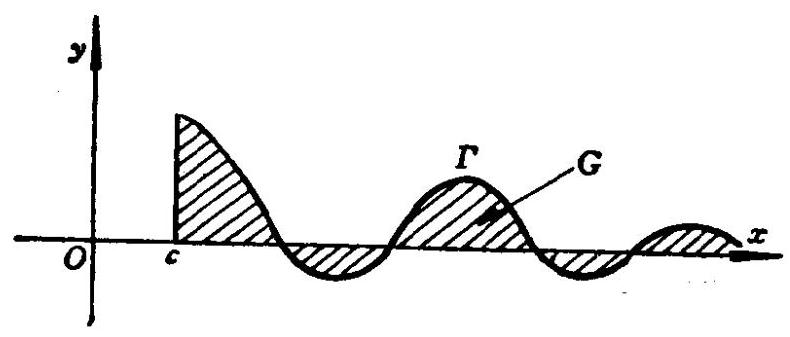
\includegraphics[max width=0.7\textwidth]{images/bo_d25ksc77aajc738obdgg_454_307_1447_790_337_0.jpg}
\end{center}
\hspace*{3em} 

图9-1

$b <  + \infty$ : 广义积分 ${\int }_{o}^{{b}^{ - }}f\left( x\right) {dx}$ 就是平面上由 $x$ 轴、直线 $x = c$ 与 $x = b$ 及函数 $f : \lbrack c,b\lbrack  \rightarrow  \mathbf{R}$ 的曲线 $\Gamma$ 所围的向正 $y$ 轴方 向无限 伸

展的平面图形 $G$ 的 “面积” (这里我们假设 $\mathop{\lim }\limits_{{d \rightarrow  {b}^{ - }}}f\left( x\right)  =  + \infty$ ).

若 ${\int }_{o}^{{b}^{ - }}f\left( x\right) {dx}$ 收敛,则 $G$ 的 “面积” 存在且有限.

若 ${\int }_{o}^{{b}^{ - }}f\left( x\right) {dx}$ 发散,则 $G$ 的 “面积” 存在但为正无穷大或负无穷大, 或根本没有 “面积”.

\begin{center}
	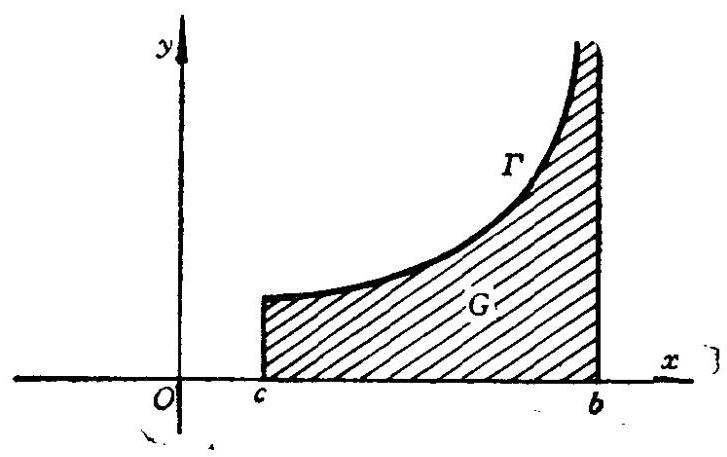
\includegraphics[max width=0.6\textwidth]{images/bo_d25ksc77aajc738obdgg_455_474_720_727_457_0.jpg}
\end{center}
\hspace*{3em} 

图 9-2

例 1 考虑广义积分 ${\int }_{0}^{+\infty }{e}^{-x}{dx}$ .

函数 $x \mapsto  {e}^{-x},x \in  \lbrack 0, + \infty \lbrack$ 连续,并且
$$\mathop{\lim }\limits_{{d \rightarrow   + \infty }}{\int }_{0}^{d}{e}^{-x}{dx} = \mathop{\lim }\limits_{{d \rightarrow   + \infty }}\left( {1 - {e}^{-d}}\right)  = 1,$$

因此广义积分 ${\int }_{0}^{+\infty }{e}^{-x}{dx}$ 收敛,并且
$${\int }_{0}^{+\infty }{e}^{-x}{dx} = 1$$

例 2 考虑广义积分 ${\int }_{1}^{+\infty }\frac{1}{x}{dx}$ .

函数 $x \mapsto  \frac{1}{x},x \in  \lbrack 1, + \infty \lbrack$ 连续,并且
$$\mathop{\lim }\limits_{{d \rightarrow   + \infty }}{\int }_{1}^{d}\frac{1}{x}{dx} = \mathop{\lim }\limits_{{d \rightarrow   + \infty }}\log d =  + \infty ,$$

故广义积分 ${\int }_{1}^{+\infty }\frac{1}{x}{dx}$ 发散,但有值
$${\int }_{1}^{+\infty }\frac{1}{x}{dx} =  + \infty .$$

例 3 考虑广义积分 ${\int }_{0}^{+\infty }\cos {xdx}$ .

函数 $x \mapsto  \cos x,x \in  \lbrack 0, + \infty \lbrack$ 连续,并且
$$\mathop{\lim }\limits_{{d \rightarrow   + \infty }}{\int }_{0}^{d}\cos {xdx} = \mathop{\lim }\limits_{{d \rightarrow   + \infty }}\sin d\text{ 不存在, }$$

故广义积分 ${\int }_{0}^{+\infty }\cos {xdx}$ 不存在,从而 ${\int }_{0}^{+\infty }\cos {xdx}$ 发散.

例 4 考虑广义积分 ${\int }_{0}^{{1}^{ - }}\frac{1}{\sqrt{1 - x}}{dx}$ 与 ${\int }_{0}^{{1}^{ - }}\frac{1}{1 - x}{dx}$ .

这里两个函数 $x \mapsto  \frac{1}{\sqrt{1 - x}},x \mapsto  \frac{1}{1 - x},x \in  \lbrack 0,1\lbrack$ 都连续, $x = 1$ 是 $f$ 的奇点,并且
\begin{align*}
	&\mathop{\lim }\limits_{{c \rightarrow  {1}^{ - }}}{\int }_{0}^{c}\frac{1}{\sqrt{1 - x}}{dx} = \mathop{\lim }\limits_{{c \rightarrow  {1}^{ - }}}{\left\lbrack  -2\sqrt{1 - x}\right\rbrack  }_{0}^{c} = 2 - \mathop{\lim }\limits_{{c \rightarrow  {1}^{ - }}}2\sqrt{1 - c} = 2,\\
	&\mathop{\lim }\limits_{{c \rightarrow  {1}^{ - }}}{\int }_{0}^{c}\frac{1}{1 - x}{dx} = \mathop{\lim }\limits_{{c \rightarrow  {1}^{ - }}}{\left\lbrack  -\log \left( 1 - x\right) \right\rbrack  }_{0}^{c} =  - \mathop{\lim }\limits_{{c \rightarrow  {1}^{ - }}}\log \left( {1 - c}\right)\\
	&=  + \infty \text{ , }
\end{align*}

因此广义积分 ${\int }_{0}^{{1}^{ - }}\frac{1}{\sqrt{1 - x}}{dx}$ 收敛,而广义积分 ${\int }_{0}^{{1}^{ - }}\frac{1}{1 - x}{dx}$ 发散,并且
$${\int }_{0}^{{1}^{ - }}\frac{1}{\sqrt{1 - x}}{dx} = 2,{\int }_{0}^{{1}^{ - }}\frac{1}{1 - x}{dx} =  + \infty .$$

2. ${\int }_{{a}^{ + }}^{c}f\left( x\right) {dx}$ 型广义积分

设 $- \infty  \leq  a < c <  + \infty$ ,函数 $f : \rbrack a,c\rbrack  \rightarrow  \mathbf{R}$ 满足下述条件:

1) $\left. {f\text{ 在 }\rbrack a,c}\right\rbrack$ 的任一有限闭区间 $\left\lbrack  {\alpha ,\beta }\right\rbrack$ 上可积,

2) 当 $a >  - \infty$ 时, $\mathop{\lim }\limits_{{x \rightarrow  {a}^{ + }}}f\left( x\right)  =  \pm  \infty$ (这时 $a$ 称为 $f$ 的奇点或瑕点).

这时,我们可以仿照 1,类似地定义 $f$ 在 $\rbrack a,c\rbrack$ 上的广义积分 ${\int }_{{a}^{ + }}^{o}f\left( x\right) {dx}$ 为:

${\int }_{{a}^{ + }}^{c}f\left( x\right) {dx}$ 存在 $\Leftrightarrow  \mathop{\lim }\limits_{{d \rightarrow  {a}^{ + }}}{\int }_{d}^{c}f\left( x\right) {dx}$ ①存在(有限或 $\pm  \infty$ )并且

这时
$${\int }_{{a}^{ + }}^{c}f\left( x\right) {dx} \triangleq  \mathop{\lim }\limits_{{d \rightarrow  {a}^{ + }}}{\int }_{d}^{c}f\left( x\right) {dx},$$

${\int }_{{a}^{ + }}^{c}f\left( x\right) {dx}$ 收敛 $\Leftrightarrow  \mathop{\lim }\limits_{{d \rightarrow  {a}^{ + }}}{\int }_{d}^{c}f\left( x\right) {dx}$ 有限,
$${\int }_{{a}^{ + }}^{c}f\left( x\right) {dx}\text{ 发散 } \Leftrightarrow  \mathop{\lim }\limits_{{d \rightarrow  {a}^{ + }}}{\int }_{d}^{o}f\left( x\right) {dx}\text{ 不存在或为 } \pm  \infty .$$

例 5 考虑广义积分 ${\int }_{{0}^{ + }}^{1}\log {xdx}$ .

这里函数 $x \mapsto  \log x,x \in  \rbrack 0,1\rbrack$ 连续, $x = 0$ 是它的唯一奇点, 由于
$$\mathop{\lim }\limits_{{d \rightarrow  {0}^{ + }}}{\int }_{d}^{1}\log {xdx} = \mathop{\lim }\limits_{{d \rightarrow  {0}^{ + }}}\left( {{\left\lbrack  x\log x\right\rbrack  }_{d}^{1} - {\int }_{d}^{1}{dx}}\right)  =  - 1,$$

故广义积分 ${\int }_{{0}^{ + }}^{1}\log {xdx}$ 收敛,其值
$${\int }_{{0}^{ + }}^{1}\log {xdx} =  - 1.$$

\footnote{
	
	① 当 $a =  - \infty$ 时, $d \rightarrow  {a}^{ + }$ 就是 $d \rightarrow   - \infty$ ,以下同.
	
}

例 6 考虑广义积分 ${\int }_{-\infty }^{0}{e}^{-x}\cos {xdx}$ .

这里函数 $x \mapsto  {e}^{-x}\cos x,x \in  \rbrack  - \infty ,0\rbrack$ 连续. $\forall d < 0$ ,直接计算得到
$${\int }_{d}^{0}{e}^{-x}\cos {xdx} = \frac{1}{2}{e}^{-d}\left( {-\sin d + \cos d}\right)  - \frac{1}{2}.$$

由此可知,极限 $\mathop{\lim }\limits_{{d \rightarrow   - \infty }}{\int }_{d}^{0}{e}^{-x}\cos {xdx}$ 不存在,因此广义积分 ${\int }_{-\infty }^{0}{e}^{-x}\cos {xdx}$ 不存在,从而发散.

3. ${\int }_{{a}^{ + }}^{{b}^{ - }}f\left( x\right) {dx}$ 型广义积分

设 $- \infty  \leq  a < b \leq   + \infty$ ,假设函数 $f : \rbrack a,b\lbrack  \rightarrow  \mathbf{R}$ 满足下述条件:

1) $f$ 在 $\rbrack a,b\lbrack$ 的任一有限闭区间 $\left\lbrack  {\alpha ,\beta }\right\rbrack$ 上可积,

2) 当 $a >  - \infty ,b <  + \infty$ 时, $\mathop{\lim }\limits_{{x \rightarrow  {a}^{ + }}}f\left( x\right)  =  \pm  \infty ,\mathop{\lim }\limits_{{x \rightarrow  {b}^{ - }}}f\left( x\right)$  $=  \pm  \infty$ (即 $a,b$ 是 $f$ 的奇点或瑕点).

现在我们假设对某一 $c \in  \rbrack a,b\lbrack$ ,广义积分之和 ${\int }_{{a}^{ + }}^{a}f\left( x\right) {dx}$  $+ {\int }_{o}^{{b}^{ - }}f\left( x\right) {dx} \in  \overline{\mathbf{R}}$ . 于是由定义可推知下面两个简单结论成立:

1) $\left. {\forall {c}^{\prime } \in  }\right\rbrack  a,b\left\lbrack  \right. ,{\int }_{{a}^{ + }}^{{a}^{\prime }}f\left( x\right) {dx} + {\int }_{{a}^{\prime }}^{{b}^{ - }}f\left( x\right) {dx} \in  \overline{\mathbf{R}}$ ,

2) ${\int }_{{a}^{ + }}^{o}f\left( x\right) {dx} + {\int }_{o}^{{b}^{ - }}f\left( x\right) {dx} = {\int }_{{a}^{ + }}^{{o}^{\prime }}f\left( x\right) {dx} + {\int }_{{o}^{\prime }}^{{b}^{ - }}f\left( x\right) {dx}$ .

2) 式表明 ${\int }_{{a}^{ + }}^{a}f\left( x\right) {dx} + {\int }_{{a}^{ - }}^{{b}^{ - }}f\left( x\right) {dx}$ 的值与 $c$ 的选择无关,因此我们引入下述定义.

定义 设函数 $f : \rbrack a,b\lbrack  \rightarrow  \mathbf{R}$ 满足上面所述条件,则 $f$ 在 $a,b\lbrack$ 上的广义积分,记为 ${\int }_{{a}^{ + }}^{b}f\left( x\right) {dx}$ ,定义为:

1) ${\int }_{{a}^{ + }}^{{b}^{\prime }}f\left( x\right) {dx}$ 存在 $\Leftrightarrow$ 对某一 $c \in  \rbrack a,b\left\lbrack  \right. ,{\int }_{{a}^{ + }}^{c}f\left( x\right) {dx}$  $+ {\int }_{c}^{{b}^{ - }}f\left( x\right) {dx}$ 是有限实数或 $\pm  \infty$ . 并且这时
$${\int }_{{a}^{ + }}^{{b}^{ - }}f\left( x\right) {dx} \triangleq  {\int }_{{a}^{ + }}^{c}f\left( x\right) {dx} + {\int }_{c}^{{b}^{ - }}f\left( x\right) {dx}.$$

2) ${\int }_{{a}^{ + }}^{{b}^{ - }}f\left( x\right) {dx}$ 收敛 $\Leftrightarrow$ 对某 $- c \in  \rbrack a,b\lbrack ,{\int }_{{a}^{ + }}^{a}f\left( x\right) {dx}$ 与 ${\int }_{c}^{{b}^{ - }}f\left( x\right) {dx}$ 收敛.

3) ${\int }_{{a}^{ + }}^{{b}^{ - }}f\left( x\right) {dx}$ 发散 $\Leftrightarrow$ 对某一 $c \in  \rbrack a,b\left\lbrack  {,{\int }_{{a}^{ + }}^{c}f\left( x\right) {dx}}\right.$ 与 ${\int }_{c}^{{b}^{ - }}f\left( x\right) {dx}$ 中至少有一个发散. 特别地

若 ${\int }_{{a}^{ + }}^{c}f\left( x\right) {dx} =  + \infty \left( {-\infty }\right) {\int }_{c}^{{b}^{ - }}f\left( x\right) {dx} =  - \infty \left( {+\infty }\right)$ ; 或 ${\int }_{{a}^{ + }}^{c}f\left( x\right) {dx}$ 与 ${\int }_{c}^{{b}^{ - }}f\left( x\right) {dx}$ 中有一个不存在,则我们称 ${\int }_{{a}^{ + }}^{{b}^{ - }}f\left( x\right) {dx}$ 不存在.

例 7 考虑广义积分 ${\int }_{-1}^{1}\frac{1}{\sqrt{1 - {x}^{2}}}{dx}$ .

这里函数 $x \mapsto  \frac{1}{\sqrt{1 - {x}^{2}}},x \in  \rbrack  - 1,1\lbrack$ 连续,并且 $x =  \pm  1$ 是它的两个奇点. 由于
\begin{align*}
	&\mathop{\lim }\limits_{{d \rightarrow   - {1}^{ + }}}{\int }_{d}^{0} - \frac{1}{1 - {x}^{2}}{dx} + \mathop{\lim }\limits_{{d \rightarrow  {1}^{ - }}}{\int }_{0}^{{d}^{\prime }}\frac{1}{\sqrt{1 - {x}^{2}}}{dx}\\
	&= \mathop{\lim }\limits_{{d \rightarrow  {1}^{ + }}}\left( {-\arcsin d}\right)  + \mathop{\lim }\limits_{{d \rightarrow  {1}^{ - }}}\left( {\arcsin {d}^{\prime }}\right)\\
	&= \frac{\pi }{2} + \frac{\pi }{2}\\
	&= \pi ,
\end{align*}

故广义积分 ${\int }_{-1}^{{1}^{ - }}\frac{1}{\sqrt{1 - {x}^{2}}}{dx}$ 收敛,并且
$${\int }_{-1}^{1} + \frac{1}{\sqrt{1 - {x}^{2}}}{dx} = \pi .$$

例 8 考虑广义积分 ${\int }_{-\infty }^{+\infty }\frac{1 + x}{1 + {x}^{2}}{dx}$ .

这里函数 $x \mapsto  \frac{1 + x}{1 + {x}^{2}},x \in  \rbrack  - \infty , + \infty \lbrack$ 连续,由于
\begin{align*}
	&{\int }_{0}^{+\infty }\frac{1 + x}{1 + {x}^{2}}{dx} = \mathop{\lim }\limits_{{d \rightarrow   + \infty }}{\int }_{0}^{d}\frac{1 + x}{1 + {x}^{2}}{dx}\\
	&= \mathop{\lim }\limits_{{d \rightarrow   + \infty }}\left( {{\left\lbrack  \operatorname{arctg}x\right\rbrack  }_{0}^{d} + \frac{1}{2}{\left\lbrack  \log \left( 1 + {x}^{2}\right) \right\rbrack  }_{0}^{d}}\right)\\
	&= \mathop{\lim }\limits_{{d \rightarrow   + \infty }}\left( {\operatorname{arctg}d + \frac{1}{2}\log \left( {1 + {d}^{2}}\right) }\right)\\
	&=  + \infty \text{ , }
\end{align*}

故广义积分 ${\int }_{-\infty }^{+\infty }\frac{1 + x}{1 + {x}^{2}}{dx}$ 发散,并且由于
\begin{align*}
	&{\int }_{-\infty }^{0}\frac{1 + x}{1 + {x}^{2}}{dx} = \mathop{\lim }\limits_{{d \rightarrow   - \infty }}{\int }_{c}^{0}\frac{1 + x}{1 + {x}^{2}}{dx}\\
	&= \mathop{\lim }\limits_{{c \rightarrow   - \infty }}\left( {{\left\lbrack  \operatorname{arctg}x\right\rbrack  }_{c}^{0} + \frac{1}{2}{\left\lbrack  \log \left( 1 + {x}^{2}\right) \right\rbrack  }_{c}^{0}}\right)\\
	&= \mathop{\lim }\limits_{{c \rightarrow   - \infty }}\left( {-\operatorname{arctg}c - \frac{1}{2}\log \left( {1 + {c}^{2}}\right) }\right)  =  - \infty ,
\end{align*}

故广义积分 ${\int }_{-\infty }^{+\infty }\frac{1 + x}{1 + {x}^{2}}{dx}$ 实际上不存在.

附注 1 如果我们在例 8 的第2个积分 ${\int }_{-\infty }^{0}\frac{1 + x}{1 + {x}^{2}}{dx}$ 计算过程中取 $c =  - d$ ,并与第一个积分的极限计算过程合并在一起,则出现下述情形:
\begin{align*}
	&\mathop{\lim }\limits_{{d \rightarrow   + \infty }}\left( {{\int }_{-d}^{0}\frac{1 + x}{1 + {x}^{2}}{dx} + {\int }_{0}^{d}\frac{1 + x}{1 + {x}^{2}}{dx}}\right)\\
	&= \mathop{\lim }\limits_{{d \rightarrow   + \infty }}\left( {{\left\lbrack  \operatorname{arctg}x\right\rbrack  }_{ - }^{d}{\left. {}_{d}^{d} + \frac{1}{2}{\left\lbrack  \log \left( 1 + {x}^{2}\right) \right\rbrack  }_{ - }^{d}\right\rbrack  }_{ - }^{d}}\right)\\
	&= \mathop{\lim }\limits_{{d \rightarrow   + \infty }}2\operatorname{arctg}d = \pi .
\end{align*}

由此似乎应推得
$${\int }_{-\infty }^{+\infty }\frac{1 + x}{1 + {x}^{2}}{dx} = \pi .$$

其实不然,因为根据广义积分 ${\int }_{a + }^{{b}^{ - }}f\left( x\right) {dx}$ 的定义,
\begin{align*}
	&{\int }_{-\infty }^{0}\frac{1 + x}{1 + {x}^{2}}{dx} + {\int }_{0}^{+\infty }\frac{1 + x}{1 + {x}^{2}}{dx} = \mathop{\lim }\limits_{{c \rightarrow   - \infty }}{\int }_{c}^{0}\frac{1 + x}{1 + {x}^{2}}{dx}\\
	&+ \mathop{\lim }\limits_{{d \rightarrow   + \infty }}{\int }_{0}^{d}\frac{1 + x}{1 + {x}^{2}}{dx}
\end{align*}

的右边 $c \rightarrow   - \infty$ 与 $d \rightarrow   + \infty$ 是两个完全独立的极限过程,而在上面我们的计算 $\mathop{\lim }\limits_{{d \rightarrow   + \infty }}\left( {{\int }_{-d}^{0}\frac{1 + x}{1 + {x}^{2}}{dx} + {\int }_{0}^{d}\frac{1 + x}{1 + {x}^{2}}{dx}}\right)$ 中,已经通过令 $c =  - d$ 而化为 $d \rightarrow   + \infty$ 的一个极限过程,从而出现两种截然不同的结果.

为了区别这种情形, 我们特作下述定义.

定义 对于广义积分 ${\int }_{{a}^{ + }}^{{b}^{ - }}f\left( x\right) {dx}$ ,

1) 若 $a =  - \infty ,b =  + \infty$ ; 则 $f$ 在 $\rbrack  - \infty , + \infty \lbrack$ 上的Cauchy广义积分主值,记为 $\left( C\right) {\int }_{-\infty }^{+\infty }f\left( x\right) {dx}$ ,定义为:
$$\text{ (C) }{\int }_{-\infty }^{+\infty }f\left( x\right) {dx} = \mathop{\lim }\limits_{{d \rightarrow   + \infty }}{\int }_{-d}^{d}f\left( x\right) {dx}\text{ . }$$

2) 若 $a >  - \infty ,b <  + \infty$ : 则 $f$ 在 $\rbrack a,b\lbrack$ 上的 Cauchy 广义积分主值,记为 $\left( C\right) {\int }_{{a}^{ + }}^{{b}^{ - }}f\left( x\right) {dx}$ ,定义为:

(C) ${\int }_{{a}^{ + }}^{{b}^{ - }}f\left( x\right) {dx} = \mathop{\lim }\limits_{{\eta  \rightarrow  {0}^{ + }}}{\int }_{a + \eta }^{b - \eta }f\left( x\right) {dx}$ .

由上述定义可知,若广义积分 ${\int }_{{a}^{ + }}^{{b}^{ - }}f\left( x\right) {dx}$ 收敛则它的值就是 Cauchy 广义积分主值 $\left( C\right) {\int }_{{a}^{ + }}^{{b}^{ - }}f\left( x\right) {dx}$ .

于是我们有
\begin{align*}
	&{\int }_{-1}^{{1}^{ + }}\frac{1}{\sqrt{1 - {x}^{2}}}{dx} = \left( C\right) {\int }_{-1}^{{1}^{ + }}\frac{1}{\sqrt{1 - {x}^{2}}}{dx} = \pi ,\\
	&{\int }_{-\infty }^{+\infty }\frac{1 + x}{1 + {x}^{2}}{dx}\text{ 发散,但 }\left( C\right) {\int }_{-\infty }^{+\infty }\frac{1 + x}{1 + {x}^{2}}{dx} = \pi .
\end{align*}

附注 2 如果出现下述形式的两个广义积分:
$${\int }_{a}^{{c}^{ - }}f\left( x\right) {dx},{\int }_{{c}^{ + }}^{b}f\left( x\right) {dx}\left( {\text{ 这里 }a >  - \infty ,b <  + \infty ,c \in  \mathbf{R}}\right)$$

则它们的和 ${\int }_{a}^{{c}^{ - }}f\left( x\right)  + {\int }_{{c}^{ + }}^{b}f\left( x\right) {dx}$ ,记为 ${\int }_{a}^{b}f\left( x\right) {dx}$ ,自然应作如下规定:

1) 广义积分 ${\int }_{a}^{b}f\left( x\right) {dx}$ 存在 $\Leftrightarrow  {\int }_{a}^{{c}^{ - }}f\left( x\right) {dx} + {\int }_{{c}^{ + }}^{b}f\left( x\right) {dx}$

为有限实数或 $\pm  \infty$ ,

并且这时
$${\int }_{a}^{b}f\left( x\right) {dx} =  - {\int }_{a}^{{c}^{ - }}f\left( x\right) {dx} + {\int }_{{c}^{ + }}^{b}f\left( x\right) {dx}.$$

2) 广义积分 ${\int }_{a}^{b}f\left( x\right) {dx}$ 收敛 $\Leftrightarrow  {\int }_{a}^{{c}^{ - }}f\left( x\right) {dx}$ 与 ${\int }_{{c}^{ + }}^{b}f\left( x\right) {dx}$

收敛.

3) 广义积分 ${\int }_{a}^{b}f\left( x\right) {dx}$ 发散 $\Leftrightarrow  {\int }_{a}^{{a}^{ - }}f\left( x\right) {dx}$ 与 ${\int }_{{a}^{ + }}^{b}f\left( x\right) {dx}$

中至少有一个发散.

4) 广义积分 ${\int }_{a}^{b}f\left( x\right) {dx}$ 的Cauchy广义积分主值

$\left( C\right) {\int }_{a}^{b}f\left( x\right) {dx} = \underset{\eta  \rightarrow  {0}^{ + }}{ \bigtriangleup  }\mathop{\lim }\limits_{{\eta  \rightarrow  {0}^{ + }}}\left( {{\int }_{a}^{c - \eta }f\left( x\right) {dx} + {\int }_{c + \eta }^{b}f\left( x\right) {dx}}\right) .$

此外,我们还可以将这种广义积分 ${\int }_{a}^{b}f\left( x\right) {dx}$ 推广到 $f$ 在 $\rbrack a$ , $b$ [上有有限个奇点的情形上去. 具体的叙述留给读者.

例 9 考虑广义积分 ${\int }_{0}^{2}\frac{x}{\sqrt{\left| 1 - {x}^{2}\right| }}{dx}$ .

这里函数 $x \mapsto  \frac{x}{\sqrt{\left| 1 - {x}^{2}\right| }},x \in  \left\lbrack  {0,2}\right\rbrack   - \{ 1\}$ 连续,并且 $x = 1$ 是它的唯一奇点. 由于
\begin{align*}
	&{\int }_{0}^{{1}^{ - }}\frac{x}{\sqrt{\left| 1 - {x}^{2}\right| }}{dx} = \mathop{\lim }\limits_{{c \rightarrow  {1}^{ - }}}{\int }_{0}^{c}\frac{x}{\sqrt{1 - {x}^{2}}}{dx} = 1,\\
	&{\int }_{1}^{2}\frac{x}{\sqrt{\left| 1 - {x}^{2}\right| }}{dx} = \mathop{\lim }\limits_{{d \rightarrow  {1}^{ + }}}{\int }_{d}^{2}\frac{x}{\sqrt{{x}^{2} - 1}}{dx} = \sqrt{3},
\end{align*}

故广义积分 ${\int }_{0}^{2}\frac{x}{\sqrt{\left| 1 - {x}^{2}\right| }}{dx}$ 收敛,并且
\begin{align*}
	&{\int }_{0}^{2}\frac{x}{\sqrt{\left| 1 - {x}^{2}\right| }}{dx} = {\int }_{0}^{1}\frac{x}{\sqrt{\left| 1 - {x}^{2}\right| }}{dx} + {\int }_{1}^{2}\frac{x}{\sqrt{\left| 1 - {x}^{2}\right| }}\\
	&= 1 + \sqrt{3}\text{ . }
\end{align*}

例 10 考虑广义积分 ${\int }_{-1}^{1}\frac{1}{x}{dx}$ .

此函数 $x \mapsto  \frac{1}{x},x \in  \left\lbrack  {-1,1}\right\rbrack   - \{ 0\}$ 连续, $x = 0$ 是它的唯一奇点. 由于
\begin{align*}
	&{\int }_{-1}^{0}\frac{1}{x}{dx} = \mathop{\lim }\limits_{{c \rightarrow  0}}{\int }_{-1}^{c}\frac{1}{x}{dx} =  - \infty ,\\
	&{\int }_{0}^{1}\frac{1}{x}{dx} = \mathop{\lim }\limits_{{d \rightarrow  {0}^{ + }}}{\int }_{d}^{1}\frac{1}{x}{dx} =  + \infty ,
\end{align*}

故广义积分 ${\int }_{-1}^{1}\frac{1}{x}{dx}$ 不存在,但是它的Cauchy广义积分主值

(C) ${\int }_{-1}^{1}\frac{1}{x}{dx} = \mathop{\lim }\limits_{{\eta  \rightarrow  {0}^{ + }}}\left( {{\int }_{-1}^{-\eta }\frac{1}{x}{dx} + {\int }_{\eta }^{1}\frac{1}{x}{dx}}\right)$
$$= 0\text{ . }$$

\section*{4. 广义积分的两个计算方法}

对广义积分, 也有类似于普通Riemann 积分的变元替换法与分部积分法. 下面我们只对 ${\int }_{c}^{{b}^{ - }}f\left( x\right) {dx}$ 型广义积分叙述这两个计算方法,对另外两种类型的广义积分,读者可以自己补充.

定理 $9 \cdot  1 \cdot  1$ (变元替换法) 设函数 $\varphi  : \lbrack \alpha ,\beta \lbrack  \rightarrow  \mathbf{R}$ 在 $\lbrack \alpha ,\beta \lbrack$ 上. 是 ${C}^{1}$ 类的, $I \subset  \mathbf{R}$ 是包含 $\varphi \left( {\lbrack \alpha ,\beta \lbrack }\right)$ 的一个区间,函数 $f : I \rightarrow  \mathbf{R}$ 在 $I$ 上连续. 那末广义积分 ${\int }_{a}^{{\beta }^{ - }}f\left( {\varphi \left( t\right) }\right) {\varphi }^{\prime }\left( t\right) {dt}$ 收敛,当且仅当极限 $\mathop{\lim }\limits_{{s \rightarrow  {\beta }^{ - }}}{\int }_{\varphi \left( a\right) }^{\varphi \left( s\right) }f\left( x\right) {dx}$ 存在并且有限. 并且这时
$${\int }_{a}^{{\beta }^{ - }}f\left( {\varphi \left( t\right) }\right) {\varphi }^{\prime }\left( t\right) {dt} = \mathop{\lim }\limits_{{s \rightarrow  {\beta }^{ - }}}{\int }_{\varphi \left( a\right) }^{\varphi \left( s\right) }f\left( x\right) {dx}.$$

证明 设 $s \in  \lbrack \alpha ,\beta \lbrack$ ,根据定积分的变元替换法 (定理 $7 \cdot  2 \cdot  3$

推论) 我们有
$${\int }_{a}^{s}f\left( {\varphi \left( t\right) }\right) {\varphi }^{\prime }\left( t\right) {dt} = {\int }_{\varphi \left( a\right) }^{\varphi \left( s\right) }f\left( x\right) {dx}.$$

两边令 $s \rightarrow  {\beta }^{ - }$ 取极限即得.

例11 计算广义积分 ${\int }_{0}^{+\infty }\frac{\operatorname{arctg}x}{{\left( 1 + {x}^{2}\right) }^{3/2}}{dx}$ .

令 $x = \varphi \left( t\right)  = \operatorname{tg}t,t \in  \left\lbrack  {0,\frac{\pi }{2}\lbrack }\right.$ . 显然 $\varphi$ 在 $\left\lbrack  {0,\frac{\pi }{2}\left\lbrack  {\text{ 上是 }{C}^{1}}\right. }\right.$ 类

的,并且 $\lbrack 0, + \infty \lbrack  = \varphi \left( \left\lbrack  {0,\frac{\pi }{2}\lbrack }\right. \right.$ ). 由于函数
$$x \mapsto  f\left( x\right)  = \frac{\operatorname{arctg}x}{{\left( 1 + {x}^{2}\right) }^{-3}},x \in  \lbrack 0, + \infty \lbrack$$

在 $\lbrack 0, + \infty \lbrack$ 上连续,故由上述定理知,
$${\int }_{0}^{+\infty }\frac{\operatorname{arctg}x}{{\left( 1 + {x}^{2}\right) }^{3/2}} - {dx}\text{ 收敛 } \Leftrightarrow  {\int }_{0}^{\frac{\pi }{2}}\frac{\operatorname{arctg}\left( {\operatorname{tg}t}\right) }{{\left( 1 + {\operatorname{tg}}^{2}t\right) }^{3/2}}{\left( \operatorname{tg}t\right) }^{\prime }{dt}\text{ 收敛. }$$

这里
$${\int }_{0}^{\frac{\pi }{2}}\frac{\operatorname{arctg}\left( {\operatorname{tg}t}\right) }{{\left( 1 + {\operatorname{tg}}^{2}t\right) }^{3/2}}{\left( \operatorname{tg}t\right) }^{\prime }{dt} = {\int }_{0}^{\frac{\pi }{2}}t\cos {tdt},$$

显然收敛,因此
\begin{align*}
	&{\int }_{0}^{+\infty }\frac{\operatorname{arctg}x}{{\left( 1 + {x}^{2}\right) }^{3/2}}{dx} = {\int }_{0}^{\frac{\pi }{2}}t\cos {tdt}\\
	&= {\left\lbrack  t\sin t\right\rbrack  }_{0}^{\frac{\pi }{2}} - {\int }_{0}^{\frac{\pi }{2}}\sin {tdt}\\
	&= \frac{\pi }{2} - 1\text{ . }
\end{align*}

定理 $9 \cdot  1 \cdot  2$ (分部积分法) 设函数 $u,v : \lbrack c,b\lbrack  \rightarrow  \mathbf{R}$ 在 $\lbrack c,b\lbrack$ 上是 ${C}^{1}$ 类的,如果

1) $\mathop{\lim }\limits_{{x \rightarrow  {b}^{ - }}}u\left( x\right) v\left( x\right)$ 存在并且有限,

2) 广义积分 ${\int }_{c}^{{b}^{ - }}{u}^{\prime }\left( x\right) v\left( x\right) {dx}$ 收敛,

则广义积分 ${\int }_{c}^{{b}^{ - }}u\left( x\right) {v}^{\prime }\left( x\right) {dx}$ 也收敛,并且
\begin{align*}
	&{\int }_{c}^{{b}^{ - }}u\left( x\right) {v}^{\prime }\left( x\right) {dx} = \mathop{\lim }\limits_{{x \rightarrow  {b}^{ - }}}\left\lbrack  {u\left( x\right) v\left( x\right)  - u\left( c\right) v\left( c\right) }\right\rbrack\\
	&- {\int }_{c}^{{b}^{ - }}{u}^{\prime }\left( x\right) v\left( x\right) {dx}
\end{align*}

证明 设 $d \in  \lbrack c,b\lbrack$ ,由定积分的分部积分法 (定理 $7 \cdot  2 \cdot  2$ 推论)我们有
\begin{align*}
	&{\int }_{c}^{d}u\left( x\right) {v}^{\prime }\left( x\right) {dx} = u\left( d\right) v\left( d\right)  - u\left( c\right) v\left( c\right)\\
	&- {\int }_{c}^{d}{u}^{\prime }\left( x\right) v\left( x\right) {dx}
\end{align*}

两边令 $d \rightarrow  {b}^{ - }$ 取极限,由定理假设知左边极限 $\mathop{\lim }\limits_{{d \rightarrow  {b}^{ - }}}{\int }_{o}^{a}u\left( x\right) {v}^{\prime }\left( x\right) {dx}$ 存在并且有限,故广义积分 ${\int }_{c}^{{b}^{ - }}u\left( x\right) {v}^{\prime }\left( x\right) {dx}$ 收敛,并且定理的等式成立.

习惯上我们把上述等式写成下述形式:
$${\int }_{c}^{{b}^{ - }}u\left( x\right) {v}^{\prime }\left( x\right) {dx} = {\left\lbrack  u\left( x\right) v\left( x\right) \right\rbrack  }_{c}^{{b}^{ - }} - {\int }_{c}^{{b}^{ - }}{u}^{\prime }\left( x\right) v\left( x\right) {dx}.$$

例 12 计算广义积分 ${\int }_{1}^{+\infty }\frac{\log x}{{x}^{2}}{dx}$ .

由于
$${\int }_{1}^{+\infty }\frac{\log x}{{x}^{2}}{dx} = {\int }_{1}^{+\infty }\log x \cdot  {\left( -\frac{1}{x}\right) }^{\prime }{dx},$$

若令函数 $u,v : \lbrack 1, + \infty \lbrack  \rightarrow  \mathbf{R}$ 为
$$\forall x \in  \lbrack 1, + \infty \lbrack ,u\left( x\right)  = \log x,v\left( x\right)  =  - \frac{1}{x}.$$

则 $u,v$ 满足分部积分法的两个条件,因此广义积分 ${\int }_{1}^{+\infty }\frac{\log x}{{x}^{2}} - {dx}$

收敛,并且
\begin{align*}
	&{\int }_{1}^{+\infty }\frac{\log x}{{x}^{2}}{dx} = {\left\lbrack  -\frac{1}{x}\log x\right\rbrack  }_{1}^{+\infty } - {\int }_{1}^{+\infty }{\left( -\frac{1}{x}\right) }_{1}^{\prime }{\left( \log x\right) }^{\prime }{dx}\\
	&= {\int }_{1}^{+\infty }\frac{1}{{x}^{2}}{dx}\\
	&= 1\text{ . }
\end{align*}

\section*{5. 两个重要的广义积分}

下面两个广义积分对判断一般广义积分的收敛与发散性将起着重要作用, 我们把它们作为一个命题列出.

命题 对广义积分 ${\int }_{{0}^{ + }}^{1}\frac{1}{{x}^{\lambda }}{dx}$ 与 ${\int }_{1}^{+\infty }\frac{1}{{x}^{\lambda }}{dx}$ 下述结论成立:

1) ${\int }_{0}^{1}\frac{1}{{x}^{\lambda }}{dx}\left\{  \begin{array}{l} \text{ 收敛,若 }\lambda  < 1; \\  \text{ 发散,若 }\lambda  \geq  1. \end{array}\right.$

2) ${\int }_{1}^{+\infty }\frac{1}{{x}^{\lambda }}{dx}\left\{  \begin{array}{l} \text{ 收敛,若 }\lambda  > 1; \\  \text{ 发散,若 }\lambda  \leq  1. \end{array}\right.$

证明 直接利用定义计算这两个积分, 即可验证命题成立.

最后作为这一节的结束,我们特作如下说明.

记号说明 为了书写简单起见,今后对广义积分 ${\int }_{0}^{{b}^{ - }}f\left( x\right) {dx}$ ! ${\int }_{{a}^{ + }}^{a}f\left( x\right) {dx}$ 及 ${\int }_{{a}^{ + }}^{{b}^{ - }}f\left( x\right) {dx}$ ,如无特别指明需要,我们一律删去上标 “ + ” 与 “ - ”,读者从 ${\int }_{a}^{b}f\left( x\right) {dx}$ 的具体形 式可以明了它是普通 Riemann积分还是广义积分.

\section*{习 题}

1. 计算下列各广义积分:

1) ${\int }_{0}^{1}\frac{x\log x}{{\left( 1 + {x}^{2}\right) }^{2}}{dx}$ , 2) ${\int }_{0}^{+\infty }\frac{{x}^{2} + 1}{{x}^{4} + 1}{dx}$ ,

3) ${\int }_{0}^{+\infty }\frac{1}{1 + {x}^{4}}{dx}$ , 4) ${\int }_{a}^{b}\frac{1}{\sqrt{\left( {x - a}\right) \left( {b - x}\right) }}{dx}$ ,

5) ${\int }_{0}^{1}\frac{1}{x\sqrt{1 + {x}^{2}}}{dx}$ , 6) ${\int }_{0}^{+\infty }\frac{{x}^{3}\log x}{{\left( 1 + {x}^{4}\right) }^{3}}{dx}$ .

2. 1) 证明: 广义积分 ${\int }_{0}^{+\infty }\frac{x - 2}{{x}^{3} - 1}{dx}$ 不存在.

2) 证明: 广义积分 ${\int }_{1}^{+\infty }\operatorname{arctg}\frac{1}{x}{dx}$ 存在但不收敛.

3) 证明: 广义积分 ${\int }_{1}^{+\infty }\frac{x\log \left( {1 + \frac{1}{x}}\right) }{1 + {x}^{2}}{dx}$ 收敛.

3. 计算下列各Cauchy广义积分主值:

1) $\left( C\right) {\int }_{0}^{+\infty }\frac{1}{1 - {x}^{2}}{dx}$ , 2) $\left( C\right) {\int }_{0}^{4}\frac{1}{{x}^{2} - {4x} + 3}{dx}$ ,

3) $\left( C\right) {\int }_{-\infty }^{+\infty }\sin {xdx}$ , 4) $\left( C\right) {\int }_{1/2}^{2}\frac{1}{x\log x}{dx}$ .

4. 计算广义积分 $I = {\int }_{0}^{+\infty }\frac{1}{\left( {1 + {x}^{2}}\right) \left( {1 + {x}^{\lambda }}\right) }{dx}\left( {\lambda  \geq  0}\right)$ .

5. 计算下列各广义积分:

1) ${\int }_{0}^{+\infty }\frac{\log x}{1 + x}{dx}$ , 2) ${\int }_{0}^{+\infty }\frac{\log x}{{\left( 1 + {x}^{2}\right) }^{2}}{dx}$ ,

3) ${\int }_{0}^{\pi }\log \left( {1 + \cos \theta }\right) {d\theta }$ , 4) ${\int }_{0}^{+\infty }\log \left( {x + \frac{1}{x}}\right) \frac{1}{1 + {x}^{2}}{dx}$ ,

5) ${\int }_{-1}^{1}\frac{{x}^{3}}{\sqrt{1 - {x}^{2}}}\log \left( \frac{1 + x}{1 - x}\right) {dx}$ , 6) ${\int }_{0}^{1}\frac{1}{{\left( 1 + x\right) }^{3}\sqrt{{x}^{2}\left( {1 - x}\right) }}{dx}$ .

\section{广义积分的收敛准则}

在上一节, 我们研究了三类广义积分:

i) ${\int }_{o}^{{b}^{ - }}f\left( x\right) {dx}$ ; ii) ${\int }_{{a}^{ + }}^{o}f\left( x\right) {dx}$ ; iii) ${\int }_{{a}^{ + }}^{{b}^{ - }}f\left( x\right) {dx}$ .

第iii) 类广义积分 ${\int }_{{a}^{ + }}^{{b}^{ - }}f\left( x\right) {dx}$ 实际上是第i) 类与第ii) 类广义积分的组合.

第ii) 类广义 积分 ${\int }_{{a}^{ + }}^{a}f\left( x\right) {dx}$ 可通过变元替换 $x =  - y$ 化为第 i) 类广义积分. 因为我们有
$${\int }_{{a}^{ + }}^{c}f\left( x\right) {dx} =  - {\int }_{{\left( -a\right) }^{ - }}^{-o}f\left( {-y}\right) {dy} = {\int }_{-o}^{{\left( -a\right) }^{ - }}f\left( {-y}\right) {dy}.$$

因此要研究一般广义积分的收敛与发散性, 实际上我们只需研究第i) 类型的广义积分 ${\int }_{o}^{{b}^{ - }}f\left( x\right) {dx}$ 的收敛与发散性.

下面我们就来研究广义积分 ${\int }_{o}^{{b}^{ - }}f\left( x\right) {dx}$ 的收敛性与发散性.

\section*{1. 广义积分的一般收敛准则}

定理 $9 \cdot  2 \cdot  1$ 设 ${\int }_{a}^{{b}^{ - }}f\left( x\right) {dx}$ 与 ${\int }_{a}^{{b}^{ - }}g\left( x\right) {dx}$ 是 任意两个广义积分.

1) 若 ${\int }_{a}^{{b}^{ - }}f\left( x\right) {dx}$ 与 ${\int }_{a}^{{b}^{ - }}g\left( x\right) {dx}$ 收敛,则广义积分 ${\int }_{a}^{{b}^{ - }}\left\lbrack  {f\left( x\right)  + g\left( x\right) }\right\rbrack  {dx}$ 也收敛,并且
$${\int }_{a}^{{b}^{ - }}\left\lbrack  {f\left( x\right)  + g\left( x\right) }\right\rbrack  {dx} = {\int }_{a}^{{b}^{ - }}f\left( x\right) {dx} + {\int }_{a}^{{b}^{ - }}g\left( x\right) {dx}.$$

2) 若 ${\int }_{a}^{{b}^{ - }}f\left( x\right) {dx}$ 收敛,则 $\forall \lambda  \in  \mathbf{R}$ ,广义积分 ${\int }_{a}^{{b}^{ - }}\left( {\lambda f}\right) \left( x\right) {dx}$ 也收敛,并且
$${\int }_{a}^{{b}^{ - }}\left( {\lambda f}\right) \left( x\right) {dx} = \lambda {\int }_{a}^{{b}^{ - }}f\left( x\right) {dx}.$$

证明 直接由广义积分的定义及函数极限的性质推出.

定理 $9 \cdot  2 \cdot  2$ (Cauchy收敛准则) 广义积分 ${\int }_{a}^{{b}^{ - }}f\left( x\right) {dx}$ 收敛的充分必要条件是:
$$\left( {\forall \bar{\varepsilon } > 0}\right) \left( {\exists B \geq  a}\right) \left( {\forall c,{c}^{\prime } \geq  B}\right)  \Rightarrow  \left| {{\int }_{c}^{{c}^{\prime }}f\left( x\right) {dx}}\right|  < \bar{\varepsilon }.$$

证明 因为广义积分 ${\int }_{a}^{{b}^{ - }}f\left( x\right) {dx}$ 收敛当且仅当函数 $F : \lbrack a,b\lbrack$  $\rightarrow  \mathrm{R}\left( {\forall c \in  \left\lbrack  {a,b\left\lbrack  \right. ,F\left( c\right)  = {\int }_{a}^{c}f\left( x\right) {dx})}\right. }\right.$ 当 $c \rightarrow  b$ 时有有限的极限存在,而 $\forall c,{c}^{\prime } \geq  a$ ,
$$F\left( \varepsilon \right)  - F\left( {c}^{\prime }\right)  = {\int }_{o}^{{o}^{\prime }}f\left( x\right) {dx}.$$

因此上述广义积分 ${\int }_{a}^{{b}^{ - }}f\left( x\right) {dx}$ 收敛的充要条件正好就是函数 $F$ 当 $c \rightarrow  {b}^{ - }$ 的Cauchy收敛准则. 从而定理成立.

定理 $9 \cdot  2 \cdot  3$ (比较判别法) 设 ${\int }_{a}^{{b}^{ - }}f\left( x\right) {dx}$ 与 ${\int }_{a}^{{b}^{ - }}g\left( x\right) {dx}$ 是任意两个广义积分,函数 $f,g : \lbrack a,b\lbrack  \rightarrow  \mathrm{R}$ 满足下述不等式:
$$\forall x \in  \lbrack a,b\lbrack ,0 \leq  f\left( x\right)  \leq  g\left( x\right) .$$

1) 若 ${\int }_{a}^{{b}^{ - }}g\left( x\right) {dx}$ 收敛,则 ${\int }_{a}^{{b}^{ - }}f\left( x\right) {dx}$ 也收敛,并且
$${\int }_{a}^{{b}^{ - }}f\left( x\right) {dx} \leq  {\int }_{a}^{{b}^{ - }}g\left( x\right) {dx}.$$

2) 若 ${\int }_{a}^{{b}^{ - }}f\left( x\right) {dx}$ 发散,则 ${\int }_{a}^{{b}^{ - }}g\left( x\right) {dx}$ 也发散.

证明 因为 $\forall x \in  \lbrack a,b\lbrack ,0 \leq  f\left( x\right)  \leq  g\left( x\right)$ ,所以
$$\forall c \in  \lbrack a,b\lbrack ,0 \leq  {\int }_{a}^{b}f\left( x\right) {dx} \leq  {\int }_{a}^{b}g\left( x\right) {dx}.$$

1) 若 ${\int }_{a}^{{b}^{ - }}g\left( x\right) {dx}$ 收敛,则由于函数 $c \mapsto  F\left( c\right)  = {\int }_{a}^{o}f\left( x\right) {dx}$  $c \in  \lbrack a,b\lbrack$ 关于 $c$ 单调上升,并且
$${\int }_{a}^{o}f\left( x\right) {dx} \leq  {\int }_{a}^{o}g\left( x\right) {dx} \leq  {\int }_{a}^{{b}^{ - }}g\left( x\right) {dx} <  + \infty ,$$

故极限 $\mathop{\lim }\limits_{{c \rightarrow  {b}^{ - }}}F\left( c\right)$ 存在且有限,从而广义积分 ${\int }_{a}^{{b}^{ - }}f\left( x\right) {dx}$ 收敛.

2) 若 ${\int }_{a}^{{b}^{ - }}f\left( x\right) {dx}$ 发散,则由反证法及结论 1) 知,广义积分 ${\int }_{a}^{{b}^{ - }}g\left( x\right) {dx}$ 必然发散.

推论 若函数 $f,g : \lbrack a,b\lbrack  \rightarrow  \mathrm{R}$ 满足条件:
$$f \geq  0,g \geq  0\text{ 并且 }f\left( x\right)  \sim  g\left( x\right) \left( {x \rightarrow  {b}^{ - }}\right) ,$$

则广义积分 ${\int }_{a}^{{b}^{ - }}f\left( x\right) {dx}$ 与 ${\int }_{a}^{{b}^{ - }}g\left( x\right) {dx}$ 有相同的收敛与发散性.

证明 因为 $f\left( x\right)  \sim  g\left( x\right) \left( {x \rightarrow  {b}^{ - }}\right)$ ,所以存在 $B,a \leq  B < b$ 使得
$$\frac{1}{2}g\left( x\right)  \leq  f\left( x\right)  \leq  {2g}\left( x\right) ,\;\forall x \in  \lbrack B,b\lbrack .$$

由此不等式及上述比较判别法立即推知此推论成立.

例 1 考虑广义积分 ${\int }_{1}^{+\infty }\frac{\log x}{\sqrt{x}}{dx}$ .

由于函数 $x \mapsto  \frac{\log x}{\sqrt{x}},x \in  \lbrack 1, + \infty \lbrack$ 在 $\lbrack 1, + \infty \lbrack$ 上连续,并且
$$\forall x \geq  e,\frac{\log x}{\sqrt{x}} \geq  \frac{1}{\sqrt{x}},$$

而广义积分 ${\int }_{1}^{+\infty }\frac{1}{\sqrt{x}}{dx}$ 发散,故由比较判别法知,广义积分

${\int }_{1}^{+\infty }\frac{\log x}{\sqrt{x}}{dx}$ 发散.

例 2 考虑广义积分 ${\int }_{1}^{+\infty }\frac{x}{\sqrt{{x}^{5} + x + 1}}{dx}$ .

函数 $x \mapsto  \frac{x}{\sqrt{{x}^{5} + x + 1}},x \in  \lbrack 1, + \infty \lbrack$ 在 $\lbrack 1, + \infty \lbrack$ 上连续,并

且由于 ${x}^{5} + x + 1 = {x}^{5}\left( {1 + \frac{1}{{x}^{4}} + \frac{1}{{x}^{5}}}\right)  \sim  {x}^{5}\left( {x \rightarrow   + \infty }\right)$ ; 故
$$\frac{x}{\sqrt{{x}^{5} + x + 1}} \sim  x \cdot  {x}^{-\frac{5}{2}} = \frac{1}{{x}^{3/2}}\left( {x \rightarrow   + \infty }\right) .$$

广义积分 ${\int }_{1}^{+\infty }\frac{1}{{x}^{3/2}}{dx}$ 收敛: 故由上述推论知,广义积分

${\int }_{1}^{+\infty }\frac{x}{\sqrt{{x}^{6} + x + 1}}{dx}$ 收敛.

例 3 考虑广义积分 ${\int }_{0}^{1}\frac{1}{\sqrt[4]{1 - {x}^{4}}}{dx}$ .

$x = 1$ 是此广义积分的唯一奇点. 并且
\begin{align*}
	&\frac{1}{\sqrt[4]{1 - {x}^{4}}} = 1/{\left\lbrack  1 - {\left( x - 1 + 1\right) }^{4}\right\rbrack  }^{\frac{1}{4}}\\
	&= 1/{\left\lbrack  4\left( 1 - x\right)  - 6{\left( 1 - x\right) }^{2} + 4{\left( 1 - x\right) }^{3} - {\left( 1 - x\right) }^{4}\right\rbrack  }^{\frac{1}{4}}\\
	&= 1/\left( {\sqrt[4]{4}{\left( 1 - x\right) }^{\frac{1}{4}}{\left\lbrack  1 - \frac{6}{4}\left( 1 - x\right)  + {\left( 1 - x\right) }^{2} - \frac{1}{4}{\left( 1 - x\right) }^{3}\right\rbrack  }^{\frac{1}{4}}}\right)\\
	&\sim  \frac{1}{\sqrt[4]{\frac{1}{4}{\left( 1 - x\right) }^{\frac{1}{4}}}}\left( {x \rightarrow  {1}^{ - }}\right)
\end{align*}

而广义积分 ${\int }_{0}^{{1}^{ - }}\frac{1}{{\left( 1 - x\right) }^{\frac{1}{4}}}{dx}$ 收敛,故广义积分 ${\int }_{0}^{{1}^{ - }}\frac{1}{\sqrt[4]{1 - {x}^{4}}}{dx}$ 收敛.

例 4 考虑广义积分 ${\int }_{0}^{+\infty }\frac{1}{{x}^{\alpha }\left( {1 + {x}^{\beta }}\right) }{dx}\left( {\alpha ,\beta  \in  \mathbf{R}}\right)$ .

$\forall \alpha ,\beta  \in  \mathbf{R}$ ,函数 $x \mapsto  \frac{1}{{x}^{\alpha }\left( {1 + {x}^{\beta }}\right) },x \in  \lbrack 1, + \infty \lbrack$ 在 $\lbrack 1, + \infty \lbrack$ 上连续.

1) $\beta  \leq  0$ : 这时
\begin{align*}
	&\frac{1}{{x}^{\alpha }\left( {1 + {x}^{\beta }}\right) } \sim  \frac{1}{{x}^{\alpha }}\left( {x \rightarrow   + \infty }\right) \text{ ,若 }\beta  < 0\text{ ; }\\
	&\frac{1}{{x}^{ * }\left( {1 + {x}^{\beta }}\right) } \sim  \frac{1}{2{x}^{\alpha }}\left( {x \rightarrow   + \infty }\right) \text{ ,若 }\beta  = 0\text{ . }
\end{align*}

因此广义积分 ${\int }_{1}^{+\infty }\frac{1}{{x}^{\alpha }\left( {1 + {x}^{\beta }}\right) }{dx}$ 收敛当且仅当 $\alpha  > 1$ .

2) $\beta  > 0$ ; 这时
$$\frac{1}{{x}^{\alpha }\left( {1 + {x}^{\beta }}\right) } \sim  \frac{1}{{x}^{\alpha  + \beta }}\left( {x \rightarrow   + \infty }\right) .$$

因此广义积分 ${\int }_{1}^{+\infty }\frac{1}{{x}^{\alpha }\left( {1 + {x}^{\beta }}\right) }{dx}$ 收敛,当且仅当 $\alpha  + \beta  > 1$ .

特别地,当 $\alpha  = 1$ 时, ${\int }_{1}^{+\infty }\frac{1}{x\left( {1 + {x}^{\beta }}\right) }{dx}$ 收敛当且仅当 $\beta  > 0$ , 并且这时
\begin{align*}
	&{\int }_{1}^{+\infty }\frac{1}{x\left( {1 + {x}^{\beta }}\right) }{dx} = {\int }_{1}^{+\infty }\frac{{x}^{\beta  - 1}}{{x}^{\beta }\left( {1 + {x}^{\beta }}\right) }{dx}\\
	&= \frac{1}{\beta }{\int }_{1}^{+\infty }\frac{1}{y\left( {1 + y}\right) }{dy}\\
	&= \frac{1}{\beta }\log 2\text{ . }
\end{align*}

\section*{2. 广义积分的绝对收敛与条件收敛}

定义 设 ${\int }_{a}^{{b}^{ - }}f\left( x\right) {dx}$ 是任一广义积分.

1) 若 ${\int }_{a}^{{b}^{ - }}\left| {f\left( x\right) }\right| {dx}$ 收敛,则称广义积分 ${\int }_{a}^{{b}^{ - }}f\left( x\right) {dx}$ 是绝对收敛的.

2) 若 ${\int }_{a}^{{b}^{ - }}\left| {f\left( x\right) }\right| {dx}$ 发散,但 ${\int }_{a}^{{b}^{ - }}f\left( x\right) {dx}$ 收敛,则称广义积分 ${\int }_{a}^{{b}^{ - }}f\left( x\right) {dx}$ 是条件收敛的.

定理 $9 \cdot  2 \cdot  4$ 任何一个绝对 收敛的广义积分 ${\int }_{a}^{{b}^{ - }}f\left( x\right) {dx}$ 是收敛的.

证明 因为 ${\int }_{a}^{b}\left| {f\left( x\right) }\right| {dx}$ 收敛,所以由定理 $9 \cdot  2 \cdot  2$ 知,
\begin{align*}
	&\left( {\forall \varepsilon  > 0}\right) \left( {\exists B \geq  a}\right) \left( {\forall c,{c}^{\prime } \geq  B}\right)  \Rightarrow  \left| {{\int }_{0}^{{c}^{\prime }}\left| {f\left( x\right) }\right| {dx}}\right|  < \bar{\varepsilon }\\
	&\Rightarrow  \left| {{\int }_{0}^{{0}^{\prime }}f\left( x\right) {dx}}\right|  < \bar{\varepsilon }.
\end{align*}

从而由同一定理知广义积分 ${\int }_{a}^{b}f\left( x\right) {dx}$ 收敛.

例 5 广义积分 ${\int }_{a}^{+\infty }\frac{\sin x}{{x}^{2}}{dx}\;\left( {a > 0}\right)$ 是绝对收敛的.

这是因为
$$\left| \frac{\sin x}{{x}^{2}}\right|  \leq  \frac{1}{{x}^{2}},{\int }_{a}^{+\infty }\frac{1}{{x}^{2}}{dx}\text{ 收敛 }\left( {a > 0}\right) .$$

例 6 广义积分 ${\int }_{{0}^{ + }}^{1}\frac{\cos \left( {x}^{2}\right) }{\sqrt{x}}{dx}$ 是绝对收敛的.

因为
$$\left| \frac{\cos \left( {x}^{2}\right) }{\sqrt{x}}\right|  \leq  \frac{1}{\sqrt{x}},{\int }_{0}^{1}\frac{1}{\sqrt{x}}{dx}\text{ 收敛. }$$

例 7 广义积分 ${\int }_{0}^{+\infty }\frac{\sin x}{{x}^{3/2}}{dx}$ 是绝对收敛的.

因为

i) 在 $\rbrack 0,1\rbrack$ 上: $\frac{\sin x}{{x}^{3/2}} \sim  \frac{1}{\sqrt{x}}\left( {x \rightarrow  {0}^{ + }}\right)$ ,广义积分 ${\int }_{0}^{1}\frac{1}{\sqrt{x}}{dx}$ 收敛,故广义积分 ${\int }_{{0}^{ + }}^{1}\frac{\sin x}{{x}^{3/2}}{dx}$ 收敛.

ii) 在 $\left\lbrack  {1, + \infty }\right\rbrack$ 上: $\left| \frac{\sin x}{{x}^{3/2}}\right|  \leq  \frac{1}{{x}^{3/2}}$ . 而广义积分 ${\int }_{1}^{+\infty }\frac{1}{{x}^{3/2}}{dx}$ 收敛,故广义积分 ${\int }_{1}^{+\infty }\left| \frac{\sin x}{{x}^{3/2}}\right| {dx}$ 收敛.

因此,广义积分 ${\int }_{{0}^{ + }}^{+\infty }\left| \frac{\sin x}{{x}^{3/2}}\right| {dx}$ 收敛,从而原广义积分 ${\int }_{0}^{+\infty }\frac{\sin x}{{x}^{3/2}}{dx}$ 绝对收敛.

例8 广义积分 ${\int }_{a}^{+\infty }\frac{\sin x}{x}{dx}$ 是条件收敛的 $\left( {a > 0}\right)$ .

1) 首先证明 ${\int }_{a}^{+\infty }\frac{\sin x}{x}{dx}$ 收敛.

为此由分部积分法, $\forall B \geq  a$ 我们有
\begin{align*}
	&{\int }_{a}^{B}\frac{\sin x}{x}{dx} = {\left\lbrack  -\frac{\cos x}{x}\right\rbrack  }_{a}^{B} - {\int }_{a}^{B}\frac{\cos x}{{x}^{2}}{dx}\\
	&= \frac{\cos a}{a} - \frac{\cos B}{B} - {\int }_{a}^{B}\frac{\cos x}{{x}^{2}}{dx}.
\end{align*}

由于 $\mathop{\lim }\limits_{{B \rightarrow   + \infty }}\frac{\cos B}{B} = 0,\mathop{\lim }\limits_{{B \rightarrow   + \infty }}{\int }_{a}^{B}\frac{\cos x}{{x}^{2}}{dx} = {\int }_{a}^{+\infty }\frac{\cos x}{{x}^{2}}{dx}$ 是绝对收敛的

(见例 5 ). 所以
$${\int }_{a}^{+\infty }\frac{\sin x}{x}{dx} = \mathop{\lim }\limits_{{B \rightarrow   + \infty }}{\int }_{a}^{B}\frac{\sin x}{x}{dx}$$

收敛.

2) 证明 ${\int }_{a}^{+\infty }\left| \frac{\sin x}{{x}^{2}}\right| {dx}$ 发散.

用反证法. 假设 ${\int }_{a}^{+\infty }\left| \frac{\sin x}{x}\right| {dx}$ 收敛. 那末由
$$\left| \frac{\sin x}{x}\right|  \geq  \frac{{\sin }^{2}x}{x} = \frac{1 - \cos {2x}}{2x},\forall x \geq  a,$$

及比较判别法知广义积分 ${\int }_{a}^{+\infty }\frac{1 - \cos {2x}}{2x}{dx}$ 收敛.

由于类似可证广义积分 ${\int }_{a}^{+\infty }\frac{\cos {2x}}{2x}{dx}$ 收敛,故由定理 $9 \cdot  2 \cdot  1$ 知, 广义积分
$${\int }_{a}^{+\infty }\frac{1}{2x}{dx} = {\int }_{a}^{+\infty }\frac{1 - \cos {2x}}{2x}{dx} + {\int }_{a}^{+\infty }\frac{\cos {2x}}{2x}{dx}$$

应该收敛,这显然是矛盾的,因为广义积分 ${\int }_{a}^{+\infty }\frac{1}{x}{dx}$ 发散. 因此广义积分 ${\int }_{a}^{+\infty }\left| \frac{\sin x}{x}\right| {dx}$ 发散.

由 1 )、2 )讨论知,广义积分 ${\int }_{a}^{+\infty }\frac{\sin x}{x}{dx}$ 是条件收敛的.

为了确定这种非绝对收敛的广义积分的收敛性, 下面我们来介绍更精细的判别法.

\section*{3. 广义积分的 Abel 与Dirichlet判别法}

为此我们首先证明下述一般性结论.

定理 $9 \cdot  2 \cdot  5$ 设函数 $f : \lbrack a,b\lbrack  \rightarrow  \mathbf{R}$ 在 $\lbrack a,b\lbrack$ 上连续,函数 $g : \lbrack a,b\lbrack  \rightarrow  \mathbf{R}$ 在 $\lbrack a,b\lbrack$ 上是 ${C}^{1}$ 类的,并且还满足下述条件:

1) 广义积分 ${\int }_{a}^{{b}^{ - }}\left| {{g}^{\prime }\left( x\right) }\right| {dx}$ 收敛.

2) 函数 $c \mapsto  F\left( c\right)  = {\int }_{a}^{b}f\left( x\right) {dx},c \in  \lbrack a,b\lbrack$ 在 $\lbrack a,b\lbrack$ 上有界.

3) $\mathop{\lim }\limits_{{c \rightarrow  {b}^{ - }}}g\left( c\right) F\left( c\right)$ 存在并且有限.

则广义积分 ${\int }_{a}^{{b}^{ - }}f\left( x\right) g\left( x\right) {dx}$ 收敛.

证明 由分部积分法, $\forall c \geq  a$ ,我们得到
\begin{align*}
	&{\int }_{a}^{c}f\left( x\right) g\left( x\right) {dx} = {\int }_{a}^{c}g\left( x\right) {F}^{\prime }\left( x\right) {dx}\\
	&= {\left\lbrack  g\left( x\right) F\left( x\right) \right\rbrack  }_{a}^{c} - {\int }_{a}^{c}F\left( x\right) {g}^{\prime }\left( x\right) {dx}\\
	&= g\left( c\right) F\left( c\right)  - g\left( a\right) F\left( a\right)  - {\int }_{a}^{c}F\left( x\right) {g}^{\prime }\left( x\right) {dx}.
\end{align*}

(*)

由假设 2 ),存在常数 $M > 0$ 使得
$$\forall x \in  \lbrack a,b\left\lbrack  {,\left| {F\left( x\right) }\right|  \leq  M}\right. \text{ . }$$

于是
$$\forall x \in  \left\lbrack  {a,b}\right\lbrack  ,\left| {F\left( x\right) {g}^{\prime }\left( x\right) }\right|  \leq  M\left| {{g}^{\prime }\left( x\right) }\right| .$$

而由假设 1 ),积分 ${\int }_{a}^{{b}^{ - }}\left| {{g}^{\prime }\left( x\right) }\right| {dx}$ 收敛,故广义积分
$${\int }_{a}^{{b}^{ - }}\left| {F\left( x\right) {g}^{\prime }\left( x\right) }\right| {dx} = \mathop{\lim }\limits_{{c \rightarrow  {b}^{ - }}}{\int }_{a}^{c}\left| {F\left( x\right) {g}^{\prime }\left( x\right) }\right| {dx}$$

收敛,从而广义积分 ${\int }_{a}^{{b}^{ - }}F\left( x\right) {g}^{\prime }\left( x\right) {dx}$ 收敛. 即极限
$$\mathop{\lim }\limits_{{a \rightarrow  {b}^{ - }}}{\int }_{a}^{b}F\left( x\right) {g}^{\prime }\left( x\right) {dx}\text{ 存在且有限. }$$

另一方面,由假设 3 ),极限 $\mathop{\lim }\limits_{{c \rightarrow  {b}^{ - }}}g\left( c\right) F\left( c\right)$ 有限. 因此由上述(*)式立即推知极限
\begin{align*}
	&\mathop{\lim }\limits_{{a \rightarrow  {b}^{ - }}}{\int }_{a}^{o}f\left( x\right) g\left( x\right) {dx} = \mathop{\lim }\limits_{{c \rightarrow  {b}^{ - }}}g\left( c\right) F\left( c\right)  - g\left( a\right) F\left( a\right)\\
	&- \mathop{\lim }\limits_{{c \rightarrow  {b}^{ - }}}{\int }_{a}^{c}F\left( x\right) {g}^{\prime }\left( x\right) {dx}
\end{align*}

存在并且有限,此即表明广义积分 ${\int }_{a}^{{b}^{ - }}f\left( x\right) g\left( x\right) {dx}$ 收敛.

推论 1 (Abel 判别法) 设函数 $f : \lbrack a,b\lbrack  \rightarrow  \mathbf{R}$ 在 $\lbrack a,b\lbrack$ 上连续,函数 $g : \lbrack a,b\lbrack  \rightarrow  \mathbf{R}$ 在 $\lbrack a,b\lbrack$ 上是 ${C}^{1}$ 类的,并且满足下述条件:

1 )函数 $g$ 在 $\lbrack a,b\lbrack$ 上单调下降且有下界.

2) 广义积分 ${\int }_{a}^{{b}^{ - }}f\left( x\right) {dx}$ 收敛.

则广义积分 ${\int }_{a}^{{b}^{ - }}f\left( x\right) g\left( x\right) {dx}$ 收敛.

证明 为此我们只需验证上述定理的条件 1)、2)、3)满足即可.

事实上,由于 $g$ 在 $\lbrack a,b\lbrack$ 上单调下降有下界,所以
$$\mathop{\lim }\limits_{{c \rightarrow  {b}^{ - }}}g\left( c\right)  = l \in  \mathbf{R},{g}^{\prime }\left( x\right)  \leq  0,\;\forall x \in  \lbrack a,b\lbrack .$$

从而 $\forall c \geq  a$ ,
$${\int }_{a}^{c}\left| {{g}^{\prime }\left( x\right) }\right| {dx} =  - {\int }_{a}^{c}{g}^{\prime }\left( x\right) {dx} = g\left( a\right)  - g\left( c\right) .$$

因此
$$\mathop{\lim }\limits_{{a \rightarrow  {b}^{ - }}}{\int }_{a}^{c}\left| {{g}^{\prime }\left( x\right) }\right| {dx} = g\left( a\right)  - \mathop{\lim }\limits_{{a \rightarrow  {b}^{ - }}}g\left( c\right)  = g\left( a\right)  - l.$$

此即表明广义积分 ${\int }_{a}^{{b}^{ - }}\left| {{g}^{\prime }\left( x\right) }\right| {dx}$ 收敛.

其次,由于广义积分 ${\int }_{a}^{{b}^{ - }}f\left( x\right) {dx}$ 收敛,并且 ${\int }_{a}^{{b}^{ - }}f\left( x\right) {dx}$  $0 \rightarrow  {3}^{ - }$  $= \lim F\left( c\right)$ ,故存在 $B,a \leq  B < b$ 使得函数 $F$ 在 $\rbrack B,b\lbrack$ 上有界. 而函数 $F$ 连续,故 $F$ 在有界闭区间 $\left\lbrack  {a,B}\right\rbrack$ 上有界,从而函数 $F$ 在 $\left\lbrack  {a,b\left\lbrack  \right. }\right.$ 上有界.

最后,极限
$$\mathop{\lim }\limits_{{c \rightarrow  {b}^{ - }}}g\left( c\right) F\left( c\right)  = \mathop{\lim }\limits_{{c \rightarrow  {b}^{ - }}}g\left( c\right)  \cdot  \mathop{\lim }\limits_{{a \rightarrow  {b}^{ - }}}F\left( c\right)  = l{\int }_{a}^{{b}^{ - }}f\left( x\right) {dx} \in  \mathbf{R}.$$

因此定理 $9 \cdot  2 \cdot  5$ 的条件全部满足,故广义积分 ${\int }_{a}^{{b}^{ - }}f\left( x\right) g\left( x\right) {dx}$ 收敛.

例 9 考虑广义积分 ${\int }_{2}^{+\infty }\frac{x\cos \left( {x}^{2}\right) }{{x}^{2} - 1}{dx}$ .

我们首先将它写成下述形式
$${\int }_{2}^{+\infty }\frac{x\cos \left( {x}^{2}\right) }{{x}^{2} - 1}{dx} = {\int }_{2}^{+\infty }\frac{{x}^{2}}{{x}^{2} - 1} \cdot  \frac{\cos \left( {x}^{2}\right) }{x}{dx}.$$

令 $g\left( x\right)  = \frac{{x}^{2}}{{x}^{2} - 1},f\left( x\right)  = \frac{\cos \left( {x}^{2}\right) }{x},\;\forall x \in  \lbrack 2, + \infty \lbrack$ .

由于
$$\text{ ① }{g}^{\prime }\left( x\right)  = {\left( \frac{{x}^{2}}{{x}^{2} - 1}\right) }^{\prime } =  - \frac{2x}{{\left( {x}^{2} - 1\right) }^{2}} < 0,\mathop{\lim }\limits_{{x \rightarrow   + \infty }}g\left( x\right)  = 1\text{ , }$$

故 $g$ 在 $\lbrack 2 + \infty \lbrack$ 上单调下降有下界.

③ 另一方面,对于广义积分 ${\int }_{1}^{+\infty }f\left( x\right) {dx} = {\int }_{2}^{+\infty }\frac{\cos \left( {x}^{2}\right) }{x}{dx}$ ,作变元替换 ${x}^{2} = y$ ,则
$${\int }_{2}^{+\infty }\frac{\cos \left( {x}^{2}\right) }{x}{dx} = \frac{1}{2}{\int }_{1}^{+\infty }\frac{\cos y}{y}{dy}.$$

用类似于例 8 的方法可证广义积分 ${\int }_{4}^{+\infty }\frac{\cos y}{y}{dy}$ 收敛,因此广义积分 ${\int }_{2}^{+\infty }f\left( x\right) {dx} = {\int }_{2}^{+\infty }\frac{\cos \left( {x}^{2}\right) }{x}{dx}$ 收敛.

根据Abel 判别法知,广义积分 ${\int }_{2}^{+\infty }\frac{x\cos \left( {x}^{2}\right) }{{x}^{2} - 1}{dx}$ 收敛.

推论 2 (Dirichlet判别法) 设函数 $f : \lbrack a,b\lbrack  \rightarrow  \mathbf{R}$ 在 $\lbrack a,b\lbrack$ 上连续,函数 $g : \lbrack a,b\lbrack  \rightarrow  \mathbf{R}$ 在 $\lbrack a,b\lbrack$ 上是 ${C}^{1}$ 类的,并且满足下述条件:

1) 函数 $g$ 在 $\left\lbrack  {a,b\left\lbrack  \right. }\right.$ 上单调下降且 $\mathop{\lim }\limits_{{x \rightarrow  {b}^{ - }}}g\left( x\right)  = 0$ .

2) 函数 $c \mapsto  F\left( c\right)  = {\int }_{a}^{c}f\left( x\right) {dx},c \in  \lbrack a,b\lbrack$ 在 $\lbrack a,b\lbrack$ 上有界. 则广义积分 ${\int }_{c}^{{b}^{ - }}f\left( x\right) g\left( x\right) {dx}$ 收敛.

证明 与推论 1 的证明一样, 我们来验证定理的条件 全部 满足.

事实上,因为 $g$ 单调下降且 $\mathop{\lim }\limits_{{x \rightarrow  {b}^{ - }}}g\left( x\right)  = 0$ ,所以
\begin{align*}
	&\mathop{\lim }\limits_{{a \rightarrow  {b}^{ - }}}{\int }_{a}^{c}\left| {{g}^{\prime }\left( x\right) }\right| {dx} = \mathop{\lim }\limits_{{c \rightarrow  {b}^{ - }}}{\int }_{a}^{c} - {g}^{\prime }\left( x\right) {dx} = g\left( a\right)  - \mathop{\lim }\limits_{{c \rightarrow  {b}^{ - }}}g\left( c\right)\\
	&= g\left( a\right) \text{ . }
\end{align*}

因此广义积分 ${\int }_{a}^{{b}^{ - }}\left| {{g}^{\prime }\left( x\right) }\right| {dx}$ 收敛.

其次由于函数 $F$ 在 $\lbrack a,b\lbrack$ 上有界,所以
$$\mathop{\lim }\limits_{{c \rightarrow  {b}^{ - }}}g\left( c\right) F\left( c\right)  = 0.$$

因此定理 $9 \cdot  2 \cdot  5$ 的全部条件满足,故广义积分
$${\int }_{a}^{b}f\left( x\right) g\left( x\right) {dx}\text{ 收敛. }$$

例10 考虑Fresnel积分
$${\int }_{0}^{+\infty }\sin \left( {x}^{2}\right) {dx}\text{ 与 }{\int }_{0}^{+\infty }\cos \left( {x}^{2}\right) {dx}.$$

设 $0 < c < b$ . 对积分 ${\int }_{o}^{b}\sin \left( {x}^{2}\right) {dx}$ 作变元替换 ${x}^{2} = y$ 得到
$${\int }_{0}^{+\infty }\sin \left( {x}^{2}\right) {dx} = \frac{1}{2}{\int }_{0}^{+\infty }\frac{\sin y}{\sqrt{y}}{dy}.$$

由此可知,我们只需讨论广义积分 ${\int }_{0}^{+\infty }\frac{\sin y}{\sqrt{y}}{dy}$ 的收敛性.

对于广义积分 ${\int }_{1}^{+\infty }\frac{\sin y}{\sqrt{y}}{dy}$ :

由于函数 $y \mapsto  g\left( y\right)  = \frac{1}{\sqrt{y}},y \in  \lbrack 1, + \infty \lbrack$ 在 $\lbrack 1 + \infty \lbrack$ 上单调

下降且 $\mathop{\lim }\limits_{{y \rightarrow   + \infty }}g\left( y\right)  = 0$ ,而函数 $c \mapsto  F\left( c\right)  = {\int }_{1}^{c}\sin {ydyc} \in  \lbrack 1, + \infty \lbrack$

在 $\lbrack 1, + \infty \lbrack$ 上以2为界. 故根据Dirichlet判别法知,广义积分 ${\int }_{1}^{+\infty }\frac{\sin y}{\sqrt{y}}{dy}$ 收敛.

对于广义积分 ${\int }_{0}^{1}\frac{\sin y}{\sqrt{y}}{dy}$ :

由于 $\left| \frac{\sin y}{\sqrt{y}}\right|  \leq  \frac{1}{\sqrt{y}},\forall y \in  \rbrack 0,1\rbrack$ ,而广义积分 ${\int }_{0}^{1}\frac{1}{\sqrt{y}}{dy}$ 收敛, 故广义积分 ${\int }_{0}^{1}\frac{\sin y}{\sqrt{y}}{dy}$ 也收敛.

因此广义积分 ${\int }_{0}^{+\infty }\frac{\sin y}{\sqrt{y}}{dy}$ 收敛,从而 Fresnel 积分 ${\int }_{0}^{+\infty }\sin \left( {x}^{2}\right) {dx}$ 收敛

同理可证, Fresnel积分 ${\int }_{0}^{+\infty }\cos \left( {x}^{2}\right) {dx}$ 收敛.

\section*{习 题}

1. 研究下列各广义积分的收敛性.

1) ${\int }_{0}^{1}\frac{1}{{x}^{2}}\sin \left( \frac{1}{{x}^{2}}\right) {dx}$ , 2) ${\int }_{0}^{1}\frac{1}{\log x}{dx}$ ,

3) ${\int }_{0}^{1}\frac{\operatorname{tg}x - 1}{\sqrt{x}}{dx}$ , 4) ${\int }_{0}^{1}\frac{\log x}{1 - {x}^{2}}{dx}$ ,

5) ${\int }_{0}^{\pi /2}\frac{\log \left( {\sin x}\right) }{\sqrt{x}}{dx}$ , 6) ${\int }_{0}^{+\infty }\frac{\sin x}{\sqrt{x + \cos x}}{dx}$ ,

7) ${\int }_{0}^{+\infty }\frac{\log \left( {1 + x}\right) }{{x}^{n}}{dx}$ , 8) ${\int }_{1}^{+\infty }\frac{1}{x}\left( {{e}^{-\frac{1}{x}} - \cos \frac{1}{x}}\right) {dx}$ .

2. 设 $\lambda  \in  R$ . 试讨论广义积分 ${\int }_{0}^{1}\frac{{x}^{\lambda } - 1}{\log x}{dx}$ 的收敛性.

3. 设 $I = {\int }_{0}^{\pi /2}\cos x\log \left( {\operatorname{tg}x}\right) {dx}$ .

1) 证明广义积分 $I$ 收敛.

2) 计算广义积分 $I$ (提示作变换 $y = \sin x$ ).

4. 设 $\lambda  \in  \mathbf{R},I = {\int }_{1}^{+\infty }{x}^{\lambda  - 1}\cos {xdx}$ .

1) 证明: 对 $\lambda  < 0$ ,广义积分 $I$ 绝对收敛.

2) 由此推出广义积分 $J = {\int }_{1}^{+\infty }{x}^{\lambda }\sin {xdx}$ 对 $\lambda  < 0$ 收敛. $J$ 绝对收敛吗?

5. 设
$$I = {\int }_{0}^{\pi /2}\log \left( {\sin x}\right) {dx},J = {\int }_{0}^{\pi /2}\log \left( {\cos x}\right) {dx}.$$

1) 证明广义积分 $I$ 与 $J$ 收敛.

2) 推导出 $I$ 与 $J$ 之间的关系式,从而计算出 $I$ 与 $J$ 的值.

6. 设 $f : \lbrack 0, + \infty \lbrack  \rightarrow  \mathrm{R}$ 满足下列条件:

1) $f \in  {C}^{2}\left( {\lbrack 0, + \infty \lbrack ,\mathrm{R}}\right)$ ,

2) ${\int }_{0}^{+\infty }{f}^{2}\left( x\right) {dx}$ 与 ${\int }_{0}^{+\infty }{\left\lbrack  {f}^{\prime \prime }\left( x\right) \right\rbrack  }^{2}{dx}$ 收敛.

试证明广义积分 ${\int }_{0}^{+\infty }{\left\lbrack  {f}^{\prime }\left( x\right) \right\rbrack  }^{2}{dx}$ 收敛.

7. 设 $\alpha  \in  {R}_{ * }^{ + }$ ,试讨论广义积分 ${\int }_{\pi }^{+\infty }\frac{\sin x}{{x}^{\alpha }}{dx}$ 的绝对收敛性.

8. 设 $P\left( x\right)  = \frac{A\left( x\right) }{B\left( x\right) }$ 是定义在 $\lbrack a, + \infty \lbrack$ 上的任一有理分式. 并且 $B\left( x\right)  > 0$ 。试研究广义积分
$$I = {\int }_{a}^{+\infty }P\left( x\right) \sin {xdx}$$

的收敛性与绝对收敛性.

(提示:证 $\deg P = \deg B - \deg A$ ,考虑以下情况:

i) $\deg P \geq  2$ , ii) $\deg P = 1$ , iii) $\deg P \leq  0$ ).

9. 设 $f : 0 + \infty \left\lbrack  { \rightarrow  R}\right\rbrack$ 是在任一有限闭区间 $\left\lbrack  {a,b}\right\rbrack   \subset  \rbrack 0, + \infty \lbrack$ 上可积的函数, $\alpha ,\beta  \in  {\mathbb{R}}_{ * }^{ + }$ ,令
$$J\left( {\alpha ,\beta }\right)  = {\int }_{0}^{+\infty }\frac{f\left( {\alpha x}\right)  - f\left( {\beta x}\right) }{x}{dx}.$$

1) 举例说明 $J\left( {\alpha ,\beta }\right)$ 可以发散.

2) 若 $a = \mathop{\lim }\limits_{{x \rightarrow  {0}^{ + }}}f\left( x\right) ,b = \mathop{\lim }\limits_{{x \rightarrow   + \infty }}f\left( x\right)$ ,计算 $J\left( {a,\beta }\right)$ 的值.

3) 若存在 $m,M \in  R$ 使得广义积分
$${\int }_{0}^{1}\frac{f\left( x\right)  - m}{x}{dx}\text{ 与 }{\int }_{1}^{+\infty }\frac{f\left( x\right)  - M}{x}{dx}$$

收敛,计算 $J\left( {\alpha ,\beta }\right)$ 的值.

4) 设 $a = \mathop{\lim }\limits_{{x \rightarrow  {0}^{ + }}}f\left( x\right)$ 并且存在 $M > 0$ 使得
$$\forall c,d \in  {R}_{ * }^{ + },\left| {{\int }_{0}^{d}f\left( x\right) {dx}}\right|  \leq  M, \mid$$

计算 $J\left( {\alpha ,\beta }\right)$ 的值.

5) 将上述结果应用到广义积分
$${\int }_{0}^{+\infty }\frac{\operatorname{arctg}{2x} - \operatorname{arctg}x}{x}{dx}\text{ 与 }{\int }_{0}^{1}\frac{x - 1}{\log x}{dx}\text{ , }$$

10. 此题是要计算广义积分
$$I = {\int }_{0}^{+\infty }\frac{\sin x}{x} \cdot  {dx}$$

的值.

1) 定义函数 $f : \left\lbrack  {0,\pi }\right\rbrack   \rightarrow  \mathrm{R}$ 如下:
$$f\left( x\right)  = \left\{  \begin{matrix} \frac{1}{x} - \frac{1}{2\sin x/2}, & \forall x \in  \rbrack 0,\pi \rbrack ; \\  0, & x = 0. \end{matrix}\right.$$

证明 $f \in  {C}^{1}\left( {\left\lbrack  {0,\pi }\right\rbrack  ,R}\right)$ .

2) 设 $n \in  N$ ,令
$${I}_{n} = {\int }_{0}^{\pi }\frac{\sin \left( {n + \frac{1}{2}}\right) x}{2\sin \frac{x}{2}}{dx}.$$

证明: ${I}_{n}$ 的值与 $n$ 无关,并计算 ${I}_{n}$ 的值.

3) 设 $\varphi  \in  {C}^{1}\left( {\left\lbrack  {0,\pi }\right\rbrack  ,R}\right)$ . 证明:积分
$${J}_{n} = {\int }_{0}^{\pi }\varphi \left( x\right) \sin \left( {n + \frac{1}{2}}\right) {xdx}$$

当 $n \rightarrow   + \infty$ 时有极限 0 .

4) 最后计算 $I = {\int }_{0}^{+\infty }\frac{\sin x}{x}{dx}$ 的值.

5) 利用 $I$ 的值证明:
$$J = {\int }_{0}^{+\infty }\frac{\sin x\cos x}{x}{dx} = \frac{\pi }{4}.$$

6) 对 $J$ 用分部积分法,证明:
$$K = {\int }_{0}^{+\infty }\frac{{\sin }^{2}x}{{x}^{2}}{dx} = \frac{\pi }{2}.$$

7) 应用恒等式 ${\sin }^{2}x + {\cos }^{2}x = 1$ ,由 $K$ 的值证明:
$$L = {\int }_{0}^{+\infty }\frac{{\sin }^{4}x}{{x}^{2}}{dx} = \frac{\pi }{4}.$$

8) 再由 $L$ 的值证明:
$$M = {\int }_{0}^{+\infty }\frac{{\sin }^{4}x}{{x}^{4}}{dx} = \frac{\pi }{3}.$$

